%%%%%%%%%%%%%%%%%%%%  練習問題（旧 prob_p37.png / prob_p38.png / prob_p39.png）  %%%%%%%%%%%%%%%%%%%%
% 第14回の［9］に続く．章単体で組んだときも番号が本体と一致するように明示しておく
% （make_chapter.sh が出す推定値より後に実行されるので，こちらが必ず勝つ）
\setcounter{qno}{9}

\filbreak
\Rank{A問題}

\Mon{基本事項の確認}

\hspace{1zw}以下の設問に答えよ．ただし気体は理想気体であるとし，気体定数を$R=8.31\U{J/mol\cdot K}$，アボガドロ数を$N_{\mathrm{A}}=6.02\times 10^{23}$\,[個/mol]とする．
\begin{komon}
\ko{1} ボルツマン定数$k_{\mathrm{B}}$はいくらか．
\ko{2} $27\Cel$における酸素分子の二乗平均速度は何$\U{m/s}$か．
\ko{3} $27\Cel$におけるヘリウム気体の1分子あたりの平均運動エネルギーは何$\U{J}$か．
\ko{4} $0.20\U{mol}$の単原子分子理想気体の温度が$10\U{K}$上昇するとき，気体の内部エネルギーの増加量は何$\U{J}$か．
\end{komon}

\filbreak
\Rank{B問題}

\Mon{気体分子運動論}\Sitei

\begin{wrapfigure}[7]{r}[0mm]{40mm}
\vspace{-4mm}
\centering
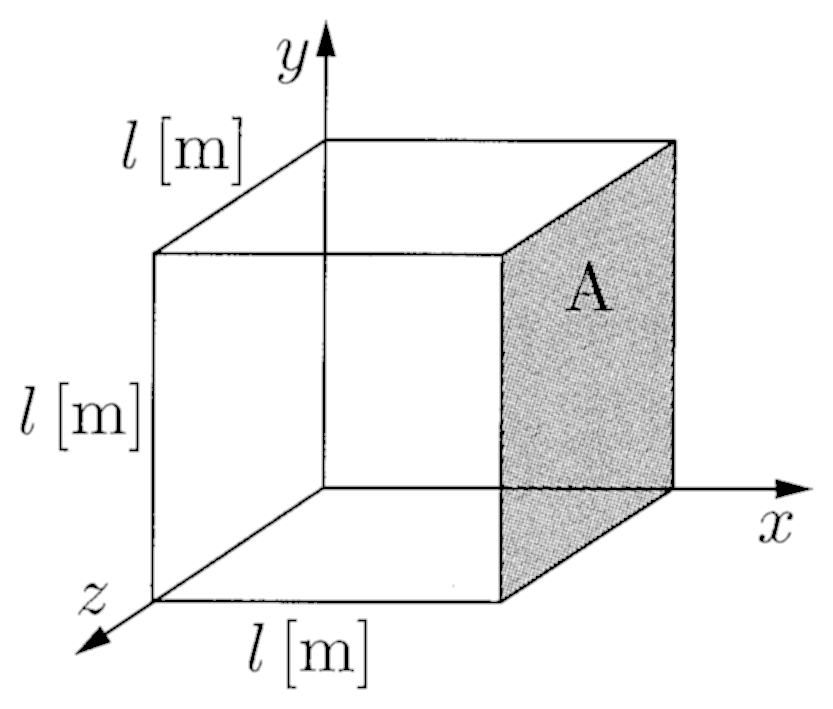
\includegraphics[keepaspectratio,width=38mm]{fig/ch15_p37_cube.png}
\end{wrapfigure}
\hspace{1zw}一辺の長さが$l\U{m}$の立方体の容器の中に，分子一個の質量が$m\U{kg}$の気体分子が$N$個入っている．右図のように$x$, $y$, $z$軸をとり，分子は互いに衝突することなく，壁と気体分子は完全弾性衝突をするものとして以下の空欄に適当な式を入れよ．必要であれば単位をつけて答えよ．

\hspace{1zw}今ある一つの分子に着目する．この分子の速さを$v\U{m/s}$，速度成分をそれぞれ$v_x\U{m/s}$, $v_y\U{m/s}$, $v_z\U{m/s}$とすれば，この分子が壁$\mathrm{A}$に衝突してはね返される際，壁$\mathrm{A}$が分子から受ける力積の大きさは，\fbox{\MARU{1}}である．よって$t\U{s}$間に壁$\mathrm{A}$がこの分子から受ける力積の大きさは，\fbox{\MARU{2}}となる．
% 誤植訂正（2026-08-31）：原本は「よってこの分子が t[s] 間に壁 A がこの分子から受ける力積の
%   大きさは」と主語が二重になっていたので，「よって t[s] 間に壁 A が…」に改めた．
ここで$N$個の分子の速さの2乗の平均値を$\overline{v^2}$，各成分の二乗の平均値をそれぞれ$\overline{v_x^2}$, $\overline{v_y^2}$, $\overline{v_z^2}$とすると，全分子が$t\U{s}$間に壁$\mathrm{A}$に及ぼす力積$I\U{N\cdot s}$は$\overline{v_x^2}$を用いて，$I=$\fbox{\MARU{3}}となる．ここで気体分子運動の等方向性および三平方の定理を利用すると，$\overline{v^2}$と$\overline{v_x^2}$の間には\fbox{\MARU{4}}の関係が成り立つから，$\overline{v^2}$を用いて$I=$\fbox{\MARU{5}}と表せる．よって壁$\mathrm{A}$が全分子から受ける力は\fbox{\MARU{6}}$\U{N}$となるから，壁$\mathrm{A}$が受ける圧力，すなわち気体の圧力$p\U{Pa}$は，$p=$\fbox{\MARU{7}}となる．したがって，容器の体積を$V\ (=l^3)\U{m^3}$とすれば，$pV=$\fbox{\MARU{8}}となる．

\Mon{気体分子運動論}

\hspace{1zw}体積$V\U{m^3}$の容器の中に，質量$m\U{kg}$の理想気体の気体分子が$N$個入っており，容器内の気体の圧力，温度はそれぞれ$p\U{Pa}$, $T\U{K}$である．気体定数を$R\U{J/mol\cdot K}$，アボガドロ定数を$N_{\mathrm{A}}\U{/mol}$とし，前問で導出したベルヌーイの式：$pV=\dfrac{Nm\overline{v^2}}{3}$を利用して以下の設問に答えよ．
\begin{komon}
\ko{1} この気体分子の二乗平均平方根速度$\sqrt{\overline{v^2}}$を，気体の温度$T$，気体定数$R$および$1\U{mol}$あたりの気体分子の質量$M\U{kg/mol}$を用いて表せ．
\ko{2} この気体分子の二乗平均平方根速度$\sqrt{\overline{v^2}}$を，圧力$p$と密度$\rho\U{kg/m^3}$を用いて表せ．
\ko{3} この気体分子1分子あたりの平均運動エネルギー$\overline{E}\U{J}$を，温度$T$とボルツマン定数$k_{\mathrm{B}}\U{J/K}$を用いて表せ．
\end{komon}

\Mon{気体分子運動論の利用}

\hspace{1zw}気体分子の運動に関する下の各問に答えよ．ただし，気体はすべて理想気体とみなしてよい．
\begin{komon}
\ko{1} 窒素ガスの分子量を28，アボガドロ定数を$6.0\times 10^{23}\U{/mol}$，気体定数を$8.3\U{J/mol\cdot K}$とする．$300\U{K}$における窒素分子の二乗平均速度を求めよ．
\ko{2} ヘリウムガス（原子量4），ネオンガス（原子量20）について，二つのガスが同じ温度のとき，1分子あたりの平均運動エネルギーの比を求めよ．
\ko{3} ヘリウムガスについて，温度が$273\Cel$になったときのヘリウム1分子あたりの平均運動エネルギーおよび二乗平均速度は$0\Cel$の時のそれぞれ何倍となるか．
\end{komon}

\Mon{内部エネルギー}\Sitei

\hspace{1zw}温度が$T\U{K}$の単原子分子理想気体が$n\U{mol}$ある．気体定数を$R\U{J/mol\cdot K}$として以下の設問に答えよ．
\begin{komon}
\ko{1} 温度を一定に保って体積を$m$倍にするとき，内部エネルギーは何倍になるか．
\ko{2} 圧力を一定に保って体積を$m$倍にするとき，内部エネルギーは何倍になるか．
\end{komon}

\begin{zuright}{38mm}
\hspace{1zw}温度が$T\U{K}$のこの気体を図のような断熱材で出来た体積$V\U{m^3}$の箱に圧力が$P\U{Pa}$となるまで封入し，ヒーターを用いて$Q\U{J}$の熱を気体に与えたところ，気体の温度は$T'\U{K}$となった．この状態変化では気体の体積が変わらないため，気体は仕事のやり取りをしない．このことを利用して，以下の設問に答えよ．
\zusep
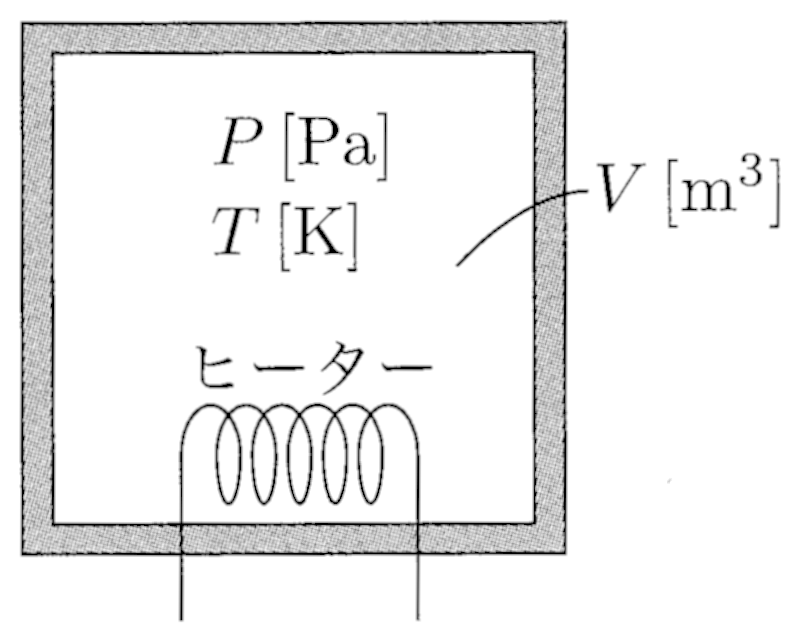
\includegraphics[keepaspectratio,width=38mm]{fig/ch15_p38_box.png}
\end{zuright}
\vspace{-\medskipamount}
\begin{komon}
\ko{3} 熱力学第一法則を用いて，気体の上昇温度$\Delta T=T'-T$を求めよ．
\ko{4} 気体の圧力$P'$を求めよ．
\end{komon}

\Mon{$p-V$図}

\begin{zuright}{40mm}
\hspace{1zw}一定量の理想気体の状態を右図の矢印の順に静かに変化させた．$\mathrm{A}$での圧力が$2p_0\U{Pa}$であるときについて，この状態変化を$p-V$図上での変化に書き直せ．ただし，グラフには$\mathrm{A}$, $\mathrm{B}$, $\mathrm{C}$点を明示し，変化の方向に矢印をつけること．
\zusep
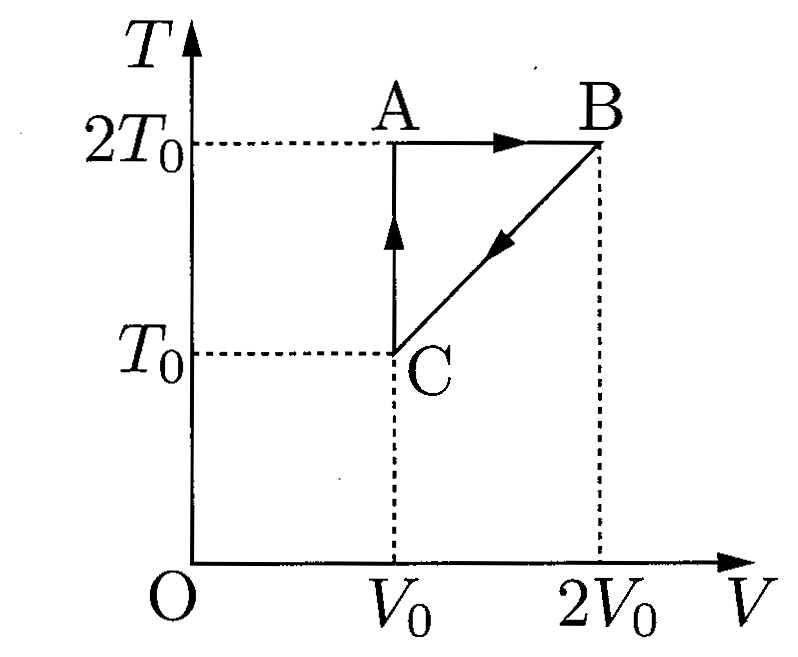
\includegraphics[keepaspectratio,width=40mm]{fig/ch15_p38_tv.png}
\end{zuright}

\filbreak
\Rank{C問題}

\Mon{球内での気体分子運動論}

\hspace{1zw}以下の空欄に適当な式を入れよ．

\begin{zuright}{40mm}
\hspace{1zw}半径$a\U{m}$の球形の容器の中に，質量$m\U{kg}$の気体分子が$N$個入っている．簡単のために，気体の各分子は一定の速さ$v\U{m/s}$で容器内を不規則な方向に飛び交っており，分子同士は互いに衝突することなく，器壁と完全弾性衝突を繰り返しているものとして考えよう．今，ある一つの分子に着目すると，この分子は器壁と衝突を繰り返して飛び回っているが，その軌跡は必ず球の中心$\mathrm{O}$を含むある一つの面内にある．これを図示したのが右図である．
\zusep
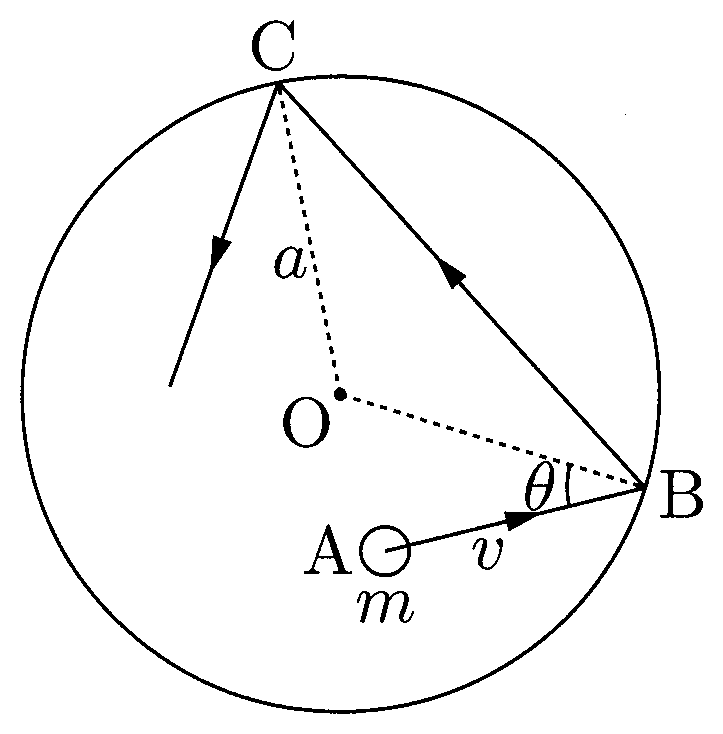
\includegraphics[keepaspectratio,width=40mm]{fig/ch15_p39_sphere.png}
\end{zuright}
% 誤植訂正（2026-08-31）：原本は「内径 a[m] の球形の容器」となっているが，図でも解答でも
%   a は中心 O から器壁までの距離（半径）として使われている（BC = 2a cosθ，S = 4πa^2，
%   V = 4πa^3/3）．内径＝直径では式が合わないので「半径」に改めた．

\hspace{1zw}さて，今，この分子が入射角$\theta$で器壁の一点$\mathrm{B}$に衝突したとすると，力積を及ぼしあう方向は半径$\mathrm{OB}$方向であるから，これに垂直な方向の速度成分は衝突の前後で変化しない．よって，衝突によるこの分子の運動量の変化は\fbox{\MARU{1}}方向に大きさ\fbox{\MARU{2}}$\U{N\cdot s}$である．次の衝突までの時間は\fbox{\MARU{3}}$\U{s}$であり，図から分かるように各回の衝突から衝突までの時間間隔は同じになるから，時間$t\U{s}$中の衝突回数は\fbox{\MARU{4}}回になる．したがって，この分子が時間$t\U{s}$中に壁面に対して与えた力積の大きさの総和は\fbox{\MARU{5}}$\U{N\cdot s}$である．

\hspace{1zw}さて，気体分子はそれぞれ運動方向が異なるため，壁面への入射角$\theta$は気体分子ごとに異なるが，(5)の答えは$\theta$に依存していない．すなわち，速度ベクトルの向きが異なる他の分子についても壁面に対して与える力積の大きさは同じになるので，$N$個の分子が時間$t\U{s}$間の間に器壁に与える力積の大きさは\fbox{\MARU{6}}$\U{N\cdot s}$となる．よって，器壁に対して及ぼす平均の力の大きさは\fbox{\MARU{7}}$\U{N}$となる．したがって容器内の圧力，つまり気体の圧力$p\U{Pa}$は\fbox{\MARU{8}}となり，また，容器の容積を$V\U{m^3}$とすると，$pV=$\fbox{\MARU{9}}と表せる．
